\documentclass[tikz,border=8pt]{standalone}

\usepackage[T1]{fontenc}
\usepackage[utf8]{inputenc}
\usepackage{lmodern}
\usetikzlibrary{arrows.meta}

\definecolor{distBlue}{RGB}{30,90,200}
\definecolor{varRed}{RGB}{176,20,30}

\begin{document}
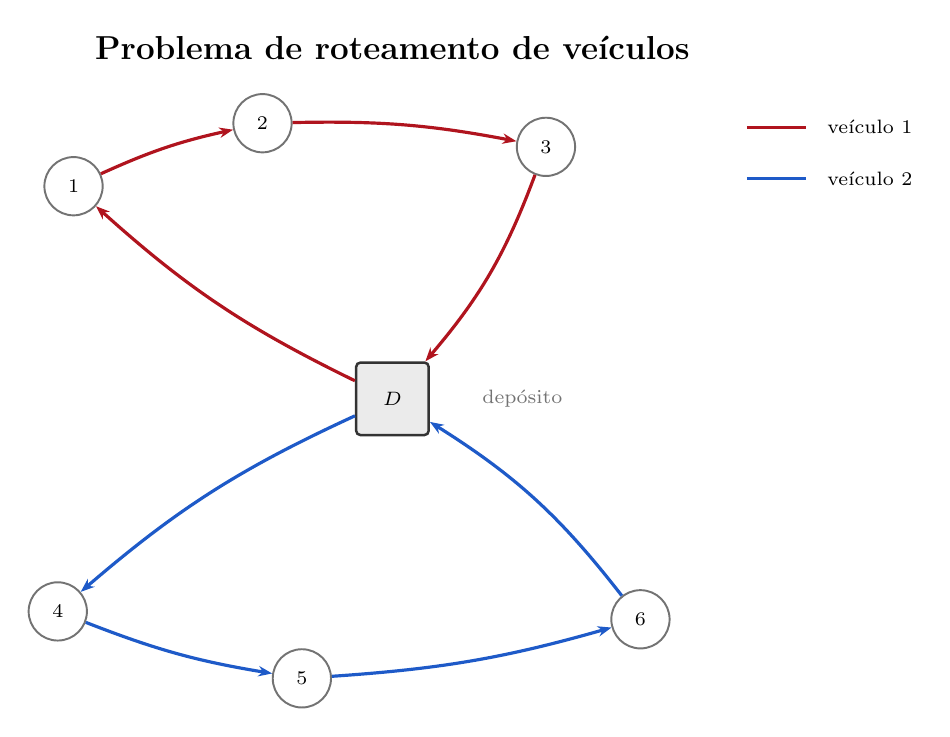
\begin{tikzpicture}[
  font=\small,
  >=Stealth,
  cliente/.style={
    circle,
    draw=black!55,
    fill=white,
    inner sep=0pt,
    minimum size=7.4mm,
    font=\scriptsize,
    line width=0.7pt,
  },
  dep/.style={
    rectangle,
    rounded corners=1.5pt,
    draw=black!80,
    fill=black!8,
    inner sep=0pt,
    minimum size=9.2mm,
    font=\scriptsize\bfseries,
    line width=0.9pt,
  },
  r1/.style={varRed, line width=1.15pt, -{Stealth[length=5pt]}},
  r2/.style={distBlue, line width=1.15pt, -{Stealth[length=5pt]}},
]

  \node[font=\bfseries\large] at (6.2,8.7)
    {Problema de roteamento de ve\'iculos};

  \node[dep] (D) at (6.2,4.25) {$D$};

  \node[cliente] (a) at (2.15,6.95) {1};
  \node[cliente] (b) at (4.55,7.75) {2};
  \node[cliente] (c) at (8.15,7.45) {3};

  \node[cliente] (e) at (1.95,1.55) {4};
  \node[cliente] (f) at (5.05,0.7) {5};
  \node[cliente] (g) at (9.35,1.45) {6};

  \draw[r1] (D) to[bend left=8] (a);
  \draw[r1] (a) to[bend left=6] (b);
  \draw[r1] (b) to[bend left=6] (c);
  \draw[r1] (c) to[bend left=10] (D);

  \draw[r2] (D) to[bend right=8] (e);
  \draw[r2] (e) to[bend right=6] (f);
  \draw[r2] (f) to[bend right=6] (g);
  \draw[r2] (g) to[bend right=10] (D);

  \node[font=\scriptsize, text=black!55] at (7.85,4.25) {dep\'osito};

  \draw[varRed, line width=1.15pt] (10.7,7.7) -- (11.45,7.7);
  \node[anchor=west, font=\scriptsize] at (11.6,7.7) {ve\'iculo 1};
  \draw[distBlue, line width=1.15pt] (10.7,7.05) -- (11.45,7.05);
  \node[anchor=west, font=\scriptsize] at (11.6,7.05) {ve\'iculo 2};

\end{tikzpicture}
\end{document}
